%!TEX root = ../thesis.tex
% ******************************* Thesis Appendix B ****************************
\chapter{Supporting work for \autoref*{chap:dst}}

% =======================================
\section{Full drug susceptibility data available}
\label{sec:full-dst}

Available phenotype information for culture-based \emph{and} line probe assay (LPA) drug susceptibility testing (DST) are shown in \autoref{tab:full-dst} and \autoref{fig:full-dst}.

\begin{table}
\centering
\begin{tabular}{|l|c|}
\hline
Drug              & Count \\ \hline
Amikacin          & 88    \\ \hline
Amikacin-LPA      & 30    \\ \hline
Capreomycin       & 51    \\ \hline
Capreomycin-LPA   & 27    \\ \hline
Ciprofloxacin-LPA & 5     \\ \hline
Ethambutol        & 90    \\ \hline
Ethambutol-LPA    & 21    \\ \hline
Isoniazid         & 98    \\ \hline
Isoniazid-LPA     & 124   \\ \hline
Kanamycin         & 51    \\ \hline
Kanamycin-LPA     & 27    \\ \hline
Moxifloxacin      & 1     \\ \hline
Moxifloxacin-LPA  & 5     \\ \hline
Ofloxacin         & 86    \\ \hline
Ofloxacin-LPA     & 30    \\ \hline
Pyrazinamide      & 1     \\ \hline
Rifampicin        & 91    \\ \hline
Rifampicin-LPA    & 124   \\ \hline
Streptomycin      & 90    \\ \hline
\end{tabular}
\caption{Culture-based and line probe assay (LPA) drug susceptibility data available for samples. The counts are the number of samples with phenotype information available for that drug.}
\label{tab:full-dst}
\end{table}

\begin{figure}
\begin{center}
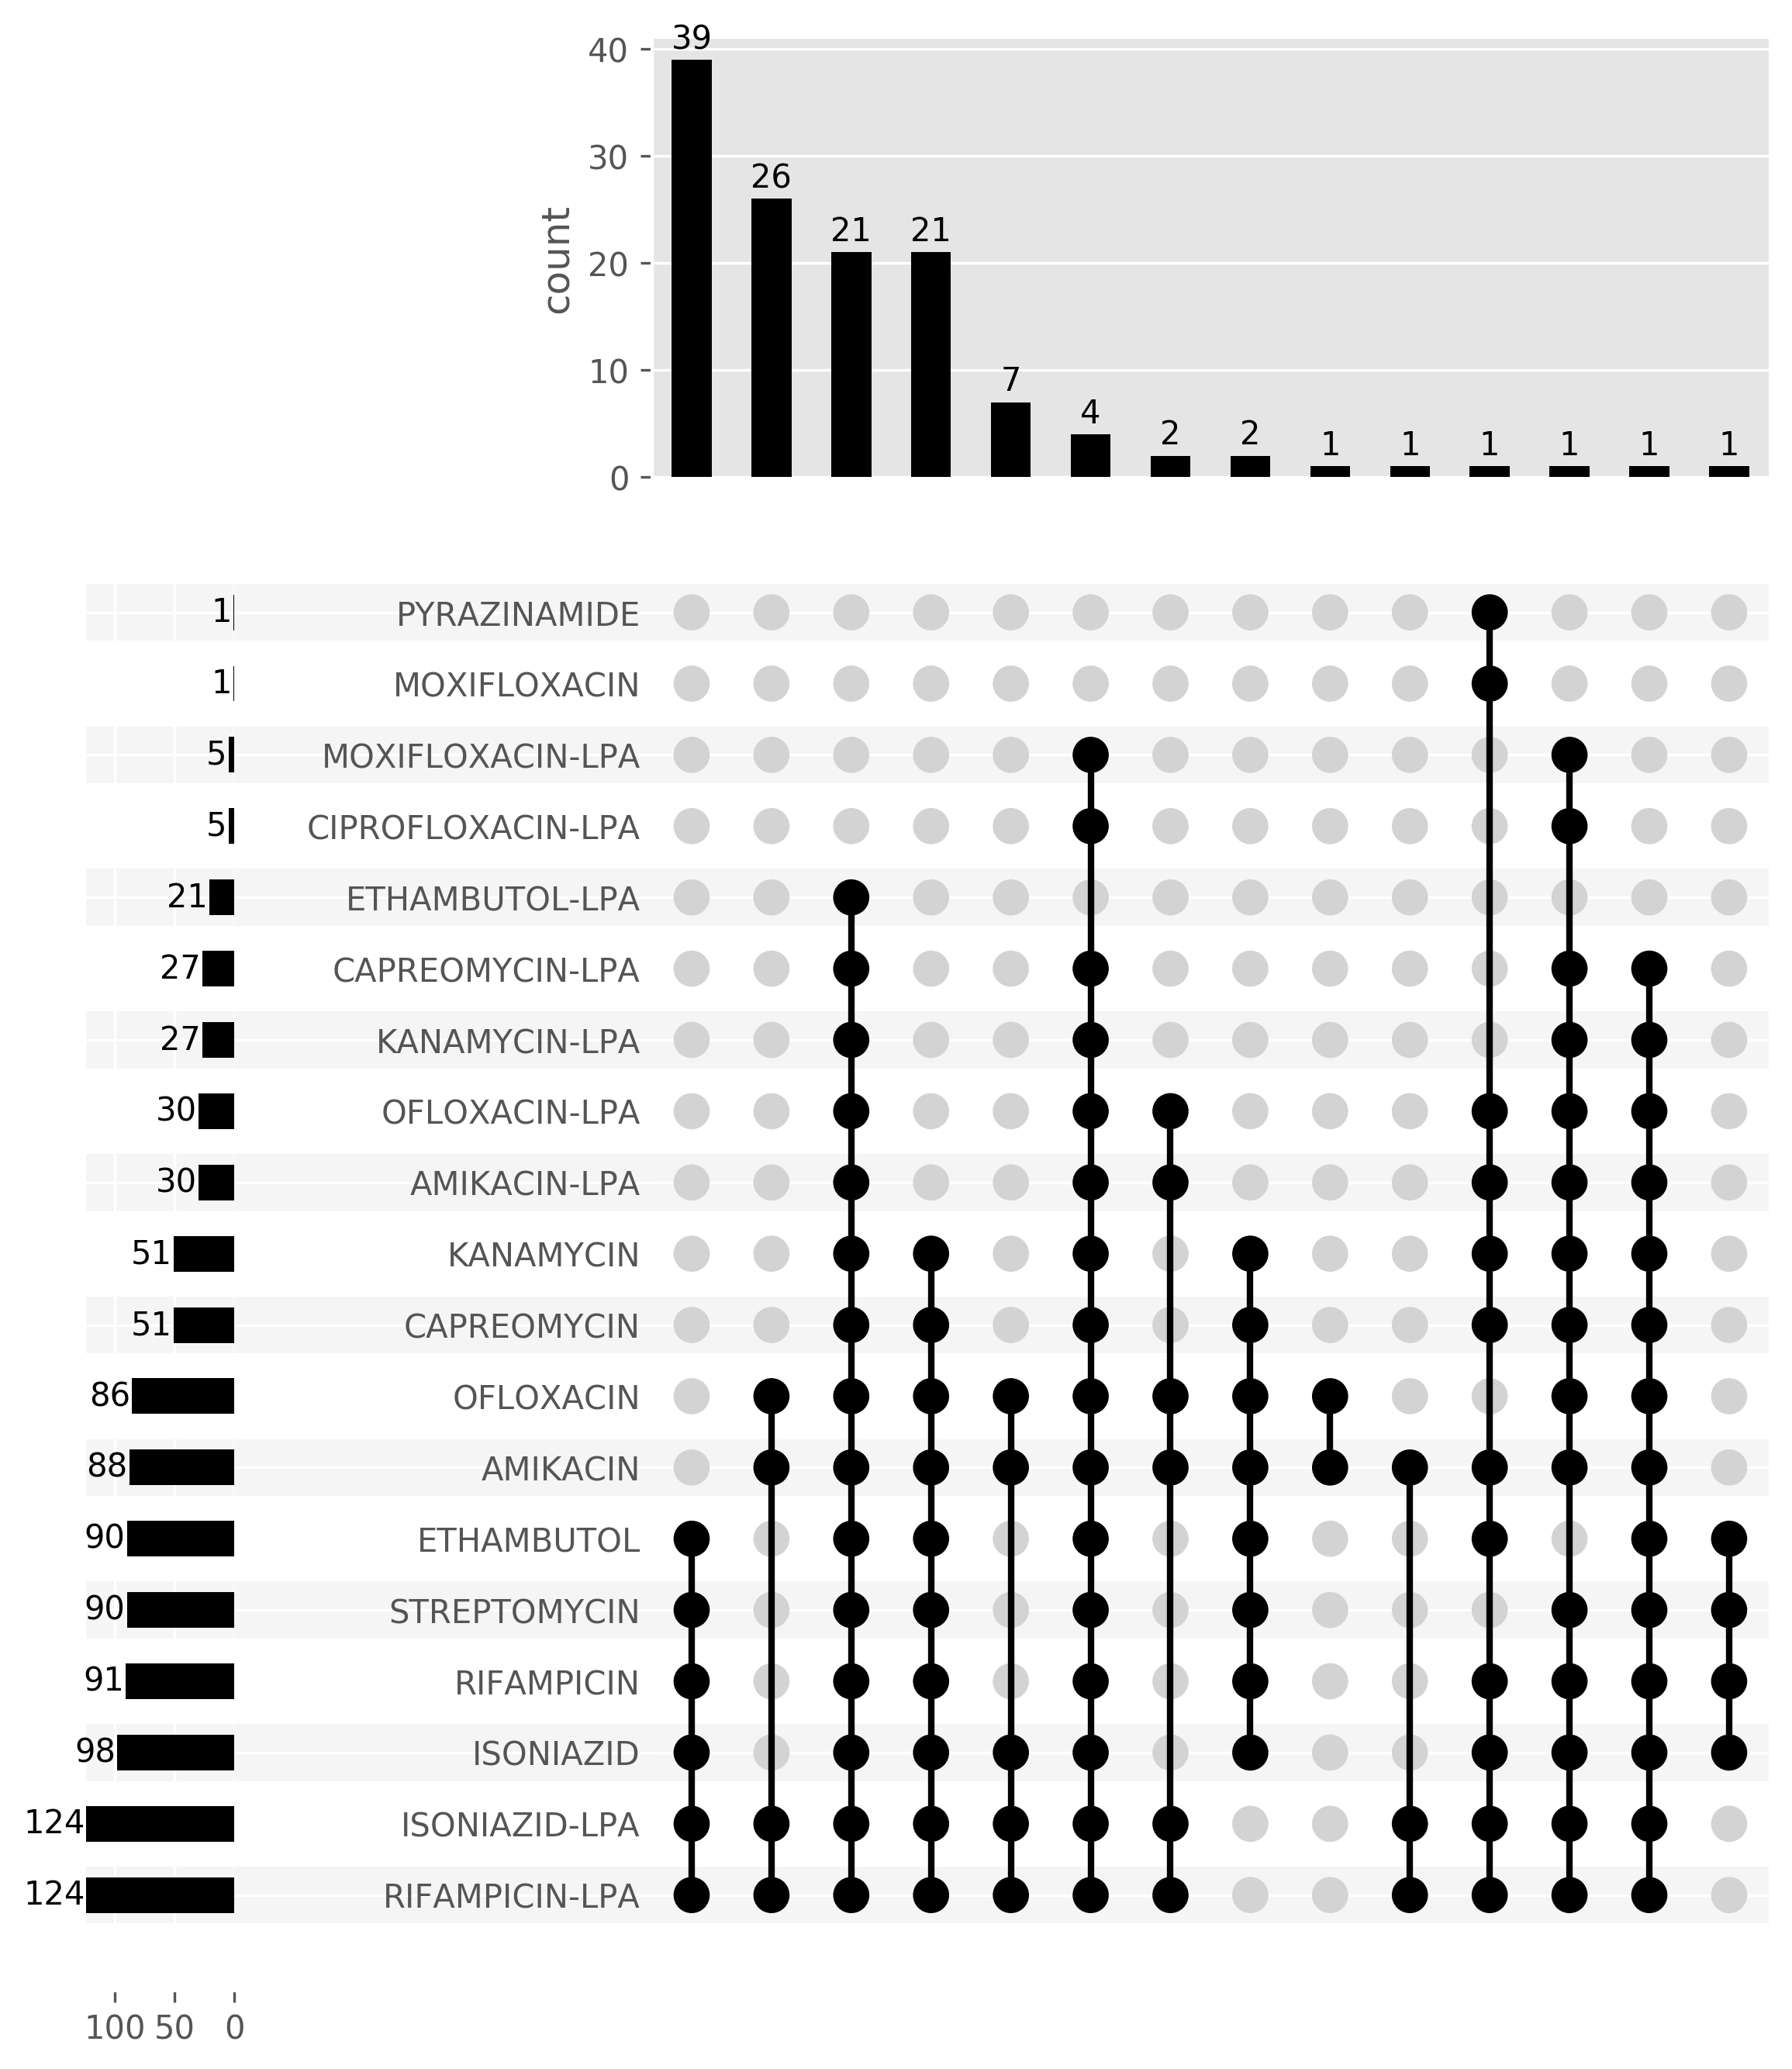
\includegraphics[width=0.90\columnwidth]{Appendix2/Figs/full-available-dst.png}
\caption{{Culture-based and line probe assay (LPA) drug susceptibility data available for samples. Each row is a drug, and the columns represent a set of samples that have phenotype information for those drugs with a filled cell. The top panel shows the number of samples in the set for that combination of drugs. The bar plot in the left panel shows the number of samples with phenotype information for that drug.
{\label{fig:full-dst}}
}}
\end{center}
\end{figure}

% ============================
\section{Constructing a panel reference graph}

\subsection{Example panel and associated VCF produced by \drprg{}}

\begin{sidewaysfigure}
% \begin{framed}
\begin{Verbatim}[frame=single,framerule=0.5mm,label=Panel,fontsize=\footnotesize]
rrs     C492X   DNA     NONE
inhA    S94A    PROT    Isoniazid
\end{Verbatim}
\begin{Verbatim}[frame=single,framerule=0.5mm,label=VCF,fontsize=\footnotesize]
##INFO=<ID=RES,Number=1,Type=String,Description="Residue the variant describes (i.e. Nucleic/Amino)">
##INFO=<ID=DRUGS,Number=.,Type=String,Description="Drugs this variant causes resistance to">
##INFO=<ID=PAD,Number=1,Type=Integer,Description="Number of bases added to start and end of gene">
##INFO=<ID=ST,Number=1,Type=String,Description="Strand the gene is on">
#CHROM  POS  ID         REF  ALT     ...         INFO
rrs     592  rrs_C492X  C    A,G,T           ... PAD=100;RES=DNA;DRUGS=NONE;ST=+
inhA    380  inhA_S94A  TCG  GCT,GCC,GCA,GCG ... PAD=100;RES=PROT;DRUGS=Isoniazid;ST=+
\end{Verbatim}
% \end{framed}
\caption{An example panel (top) expected by \drprg{}. The columns indicate the gene, mutation, residue the variant describes, and drug the entry impacts. The panel is turned into a VCF (bottom) with proteins converted to DNA. Associated information from the panel and annotation are encoded in the INFO field for each entry. Note: some information not necessary for this example is removed from the VCF entry shown here to reduce the size.}
\label{fig:example-panel}
\end{sidewaysfigure}

\subsection{Panel-based \prg{} density and haplotype problems}
\label{app:panel-prg-issues}

% add in some examples of crazy sites that lead to the change in construction method
% use the example of the S95T susceptible mutation that uncovered this problem